\begin{song}{title=\predtitle\centering Hercegovina \\\large \vspace*{-0.3cm}}  %% sem se napíše jméno songu a autor
\nejnejvetsi

\begin{centerjustified}

\sloka
	/: ^*{G}He  rcegovina, cha-cha-cha-ju-cha-cha,
	
	^{D\,\,}lautr rovina, cha-cha-cha-ju-cha-cha, :/
	
	/: ^{G}tu musela ^*{C}vy bojovat ^{D{\color{white}\_\_\_}G\,}infanteria, cha-cha. :/
	
\sloka
	/: ^*{G}In fanteria, cha-cha-cha-ju-cha-cha,
	
	^{D\z}čestná setnina, cha-cha-cha-ju-cha-cha, :/
	
	/: ^{G\z}ta~musela ^{C\z}bojovati ^{D}za císaře ^{\z G}pána, cha-cha. :/
	
\sloka
	/: ^{G\z}Za císaře pána, cha-cha-cha-ju-cha-cha,
	
	^{D\z}a~jeho rodinu, cha-cha-cha-ju-cha-cha :/
	
	/: ^{G\z}museli jsme ^{C\z}vybojovat ^{D\z G}Hercegovinu, cha-cha. :/
	
\sloka
	/: ^{G\z}Vzhůru po stráni, š š š š š,
	
	^{D\z}šnelcuk uhání, š š š š š, :/
	
	/: ^{G\z}a~pod strání ^{C\z}jsou schováni ^{D\z G}Mohamedáni, cha-cha. :/

\end{centerjustified}
\newpage
\begin{centerjustified}
\sloka
	/: ^{G\z}Mohamedáni, cha-cha-cha-ju-cha-cha,
	
	^{D\z}to~jsou pohani, cha-cha-cha-ju-cha-cha, :/
	
	/: ^{G\z}kalhoty maj ^{C\z}roztrhaný a ^{D\z}smrkaj do ^{\z G}dlaní, cha-cha. :/
	
\sloka
	/: ^{G\z}Tyhle Turkyně, cha-cha-cha-ju-cha-cha,
	
	^{D\z}tlustý jak dýně, cha-cha-cha-ju-cha-cha. :/
	
	/: ^{G\z}Císař pan je ^{C\z}nerad vidí ^{D\z}ve svý ^{\z G}rodině, cha-cha. :/
	
\sloka
	/: ^{G\z}Tuto píseň skládal, cha-cha-cha-ju-cha-cha,
	
	^{D\z}jeden hoch mladý, cha-cha-cha-ju-cha-cha, :/
	
	/: ^{G\z}který se dal ^{C\z}skrz svou holku k ^{D\z G}infanterii, cha-cha. :/
	

\end{centerjustified}
\setcounter{Slokočet}{0}
\end{song}


\begin{figure}[h]
\predtitle\centering
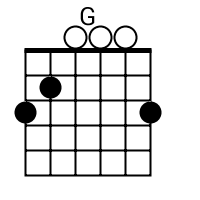
\includegraphics[width=3cm]{../Akordy/g.png}
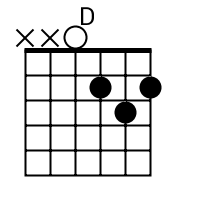
\includegraphics[width=3cm]{../Akordy/d.png}
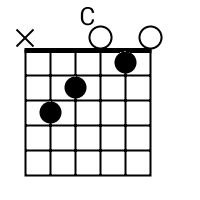
\includegraphics[width=3cm]{../Akordy/c.png}
\end{figure}
